\documentclass[11pt]{beamer}
\title{Synthesizing Ranking Functions from Bits and Pieces}
\usepackage{verbatim}
\usepackage{amsmath}
\usepackage{amsthm}
\usepackage{listings}
\usepackage{graphics}
\usepackage{color}
\usepackage{multicol}
\usepackage{stmaryrd}\usefonttheme[onlymath]{serif}

\newtheorem{proposition}{Proposition}
\author{Caterina Urban et al.}
\date{\today}


\begin{document}
\maketitle
\begin{frame}\frametitle{Overview}

\begin{itemize}
\item Synthesizing ranking function to prove termination based on safety checking.
\item Bits: \textbf{bits} of information from terminating executions. 

Pieces: Extrapolate from these bits to obtain ranking functions \textbf{pieces} and combine them into ranking functions.

\item Algorithm implemented in \textsc{SeaHorn} targeting on C code.

\end{itemize}
\end{frame}

\begin{frame}\frametitle{Overview}
\begin{center}
\includegraphics[scale=0.26]{Overview.png}
\end{center}
\end{frame}

\begin{frame}\frametitle{Preliminaries}
\begin{itemize}
\item Transition System: $\langle \Sigma ,\tau\rangle$: states and transition relation.
\item $s\in \Sigma$ is a pair $\langle l, \bar{x}\rangle$ where $l$ is program control point and $\bar{x}$ is the vector of values of variables.
\item A state is \textit{terminating}, \textit{non-terminating}, \textit{potentially terminating} and \textit{potentially nonterminating}.
\item Ranking function: $\forall s,s'. \tau(s, s')\Rightarrow rank(s') < rank(s)$, $\forall s. rank(s) \ge 0$.
\item Control flow graph induced by the transition system.
\end{itemize}

\end{frame}

\begin{frame}\frametitle{Loops in Control Flow Graph}
\begin{itemize}
\item Loop header, entry e	dge, loop edge and exit edge.
\end{itemize}

\begin{center}
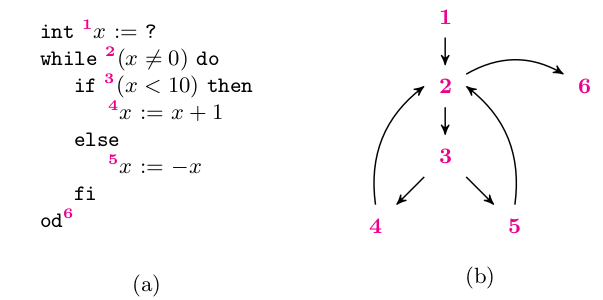
\includegraphics[scale=0.4]{cfgloops.png}
\end{center}
\end{frame}

\begin{frame}\frametitle{Verifying Safety Properties}
Verifying Nontermination: 
\begin{center}
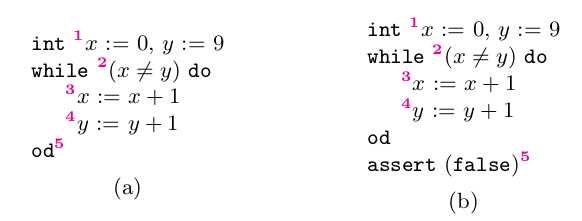
\includegraphics[scale=0.4]{vnt.png}
\end{center}

Verifying a ranking function: 
\begin{center}
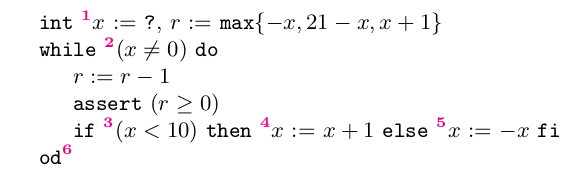
\includegraphics[scale=0.4]{vrf.png}
\end{center}

\end{frame}

\begin{frame}\frametitle{Verifying Termination via Safety: the Algorithm}

\begin{center}
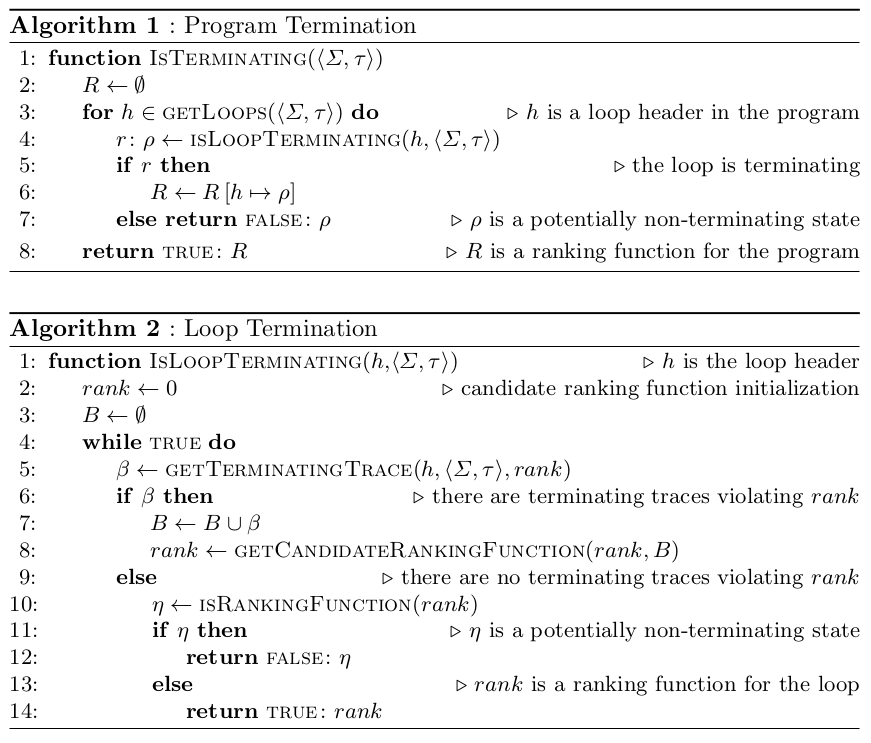
\includegraphics[scale=0.33]{algo.png}
\end{center}

\end{frame}

\begin{frame}
\frametitle{Verifying Termination via Safety}
\begin{center}
\includegraphics[scale=0.26]{Overview.png}
\end{center}
\end{frame}

\begin{frame}\frametitle{Search for Ranking Function Counterexamples}
$\mathbf{T_{TERM}}$\textbf{Transformation}: For a program $\langle \Sigma, \tau\rangle $ and candidate ranking function $rank$. Construct new set of state $\Sigma' = (\Sigma \times \mathbb{Z}) \cup \{\omega\}$, and modified transition relation $\tau'$:
\begin{itemize}
\item  For each loop entry transition $\tau(s, \langle h, \bar{x} \rangle )$, there exists an $\tau^{rank}$ s.t.
\[\tau^{rank}(\langle s,r\rangle, \langle\langle h, \bar{x}\rangle, r' \rangle) \Leftrightarrow \tau(s, \langle h, \bar{x}\rangle) \wedge r' = rank(\bar{x})\]

\item For each loop transition $tau(\langle h, \bar{x} \rangle, s)$, there exists a loop transition $r^{\ominus}$ s.t.
\[r^{\ominus}(\langle\langle h, \bar{x}\rangle, r\rangle, \langle s, r'\rangle)\Leftrightarrow \tau(\langle h, \bar{x}\rangle, s) \wedge r' = r \ominus 1\]

\item For each loop exit transition $\tau(s, s')$, there exists a transition $\tau^{<}$ to the error state $\omega$ s.t.
\[\tau^{<}(\langle s,r\rangle, \omega) \stackrel{def}{=} r < 0\]
\end{itemize}


\end{frame}
\begin{frame}\frametitle{Example: $\mathbf{T_{TERM}}$ Transformation}

\begin{center}
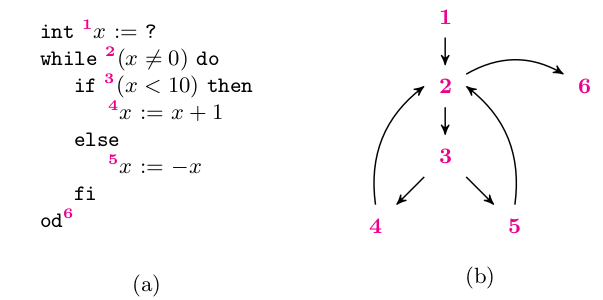
\includegraphics[scale=0.4]{cfgloops.png}
\end{center}

\begin{center}
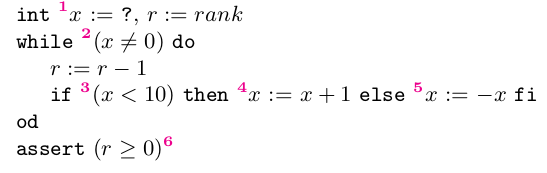
\includegraphics[scale=0.4]{tterm.png}
\end{center}

\end{frame}

\begin{frame}\frametitle{Search for Ranking Function Counterexamples}

\begin{theorem}
The error state $\omega$ is reachable

iff.

A finite trace jump out of loop with header $h$ and visit $h$ more than $rank(\bar{x})$ times.

\end{theorem}
\end{frame}

\begin{frame}\frametitle{Validating Ranking Function}

$\mathbf{T_{RANK}}$ \textbf{Transformation}:

\[\tau^{rank}(\langle s,r\rangle, \langle\langle h, \bar{x}\rangle, r' \rangle) \Leftrightarrow \tau(s, \langle h, \bar{x}\rangle) \wedge r' = rank(\bar{x})\]

\[r^{\ominus}(\langle\langle h, \bar{x}\rangle, r\rangle, \langle s, r'\rangle)\Leftrightarrow \tau(\langle h, \bar{x}\rangle, s) \wedge r' = r \ominus 1\]

For \textbf{loop transitions} $\tau(s, s')$.
\[\tau^{<}(\langle s,r\rangle, \omega) \stackrel{def}{=} r < 0\]
\end{frame}

\begin{frame}\frametitle{Example: $\mathbf{T_{RANK}}$ Transformation}
\begin{center}
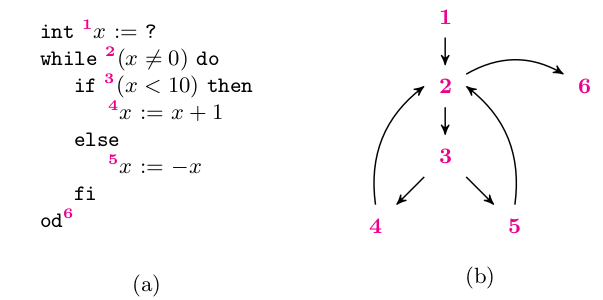
\includegraphics[scale=0.4]{cfgloops.png}

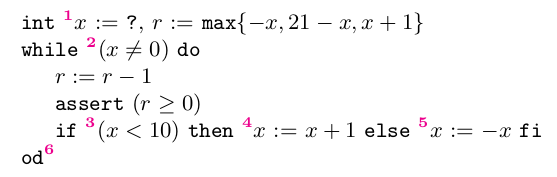
\includegraphics[scale=0.4]{trank.png}
\end{center}
\end{frame}

\begin{frame}\frametitle{Validating Ranking Functions}

\begin{theorem}
The error state $\omega$ is reachable 

iff.

The corresponding finite trace is the prefix of a an infinite trace which visits the loop header $h$ more than $rank(\bar{x})$ times.
\end{theorem}

\end{frame}


\begin{frame}\frametitle{Synthesis of Candidate Ranking Function}

\begin{itemize}

\item Target: affine ranking function pieces.

\item $\{\langle\bar{x}_1, r_1\rangle, \langle \bar{x}_2, r_2\rangle, \ldots\}$ is the set of pairs mapping the initial states of terminating traces to number of iterations need for termination.

\item Template: $\bar{m}\cdot \bar{x} + q$
\end{itemize}
\begin{center}
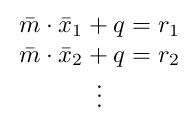
\includegraphics[scale=0.4]{affine.png}
\end{center}

Then utilize these ranking pieces to form piecewise, multi-phase and lexicographic ranking functions.

\end{frame}



\begin{frame}\frametitle{Implementation and Experiments}

Implemented in \textsc{SeaHorn}. 

Experimental evaluation is conducted on SV-COMP 2015. 

\begin{center}
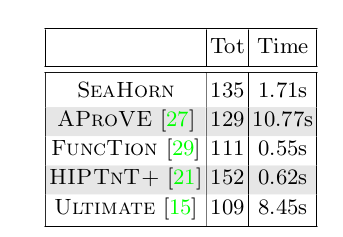
\includegraphics[scale=0.4]{gen.png}
\end{center}

\end{frame}

\begin{frame}\frametitle{Experimental Evaluation}

\begin{center}
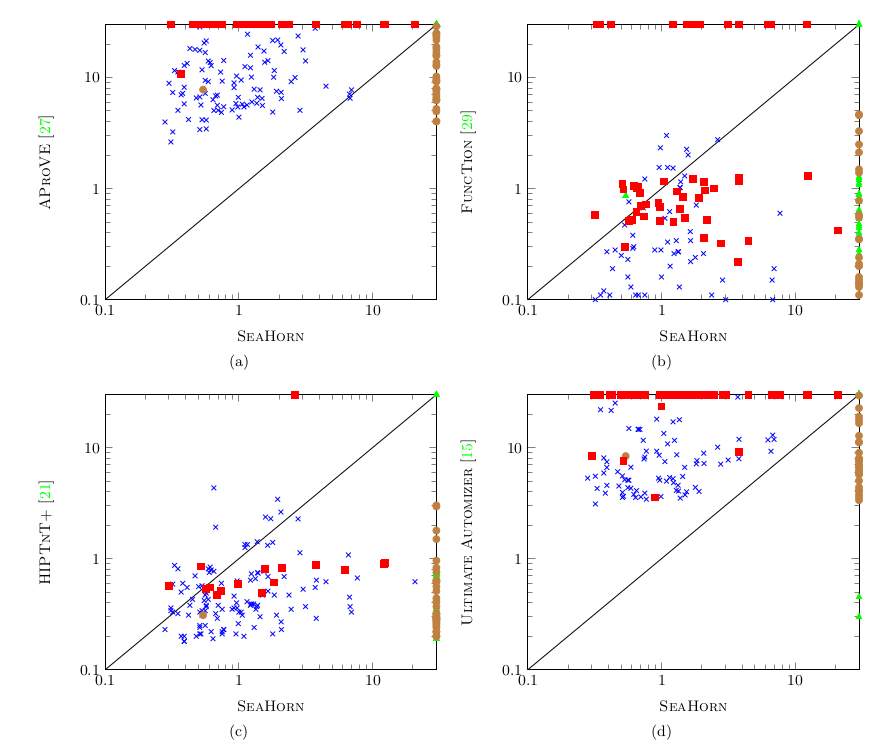
\includegraphics[scale=0.34]{experi.png}
\end{center}
\end{frame}



\end{document}